\documentclass[a4paper, 12pt]{article}
\usepackage[OT1]{fontenc}
\usepackage{ngerman}
\usepackage[latin1]{inputenc}
\usepackage{graphics}
\usepackage{fancyhdr}
\usepackage{epsfig}
\usepackage{abstract}
% nur f�r linux's pdflatex
%\usepackage{pdfpages}

\begin{document}

%definitionen
\newenvironment{code}
	{\begin{tabbing}}
	{\end{tabbing}}

% Kopfzeile mit Kapitel
\renewcommand{\sectionmark}[1]{\markleft{#1}{}}
\pagestyle{fancyplain}
\rhead{\footnotesize\thepage}
\lhead{\footnotesize\leftmark}
\cfoot{}

%Titelseite
\begin{titlepage}
\title{
\includegraphics[width=7cm]{../res/uniol.jpg}\\ \vspace{2cm}				
			\textbf{Entwicklung eines Frameworks zur Simulation von Komponentennetzwerken\\}
			{ \large Ausarbeitung zum Individuellen Projekt\\ \vspace{2cm}}}
			
\author{Marko Hoyer\\Hans-Fleischer Stra�e 29-31\\26133 Oldenburg\\
				Marko.Hoyer@informatik.uni-oldenburg.de
				}

\maketitle

\vspace{2cm}
\textbf{Betreuer: } \parbox[t]{7cm}{Jun.-Prof. Dr. Ralf Reussner\\Dipl.-Wirtsch.-Inform. Steffen Becker}

\thispagestyle{empty}
\end{titlepage}

\thispagestyle{empty}
The abstract (100-200 Words).
\newpage

%Inhaltsverzeichnis
\tableofcontents
\thispagestyle{empty}
\newpage

\section{Einleitung}
\label{sec:einleitung}

\subsection{Motivationen und Hintergr�nde}
\label{sec:einleitung:motivation}
Soll ein neu zu erstellendes Softwaresystem auf Basis vorhandener Komponenten erstellt werden, so stellt sich h�ufig die Frage nach der Performance des Gesamtsystems. Deren Beantwortung vor der Implementierung ist h�ufig Voraussetzung zur Einhaltung einiger nichtfunktionaler Anforderungen wie zum Beispiel der mittleren Antwortzeit. Werden die Antwortzeiten der Dienste der einzelnen Komponenten als bekannt vorausgesetzt, so gilt es nun, die Antwortzeit des Gesamtsystems mit einer bestimmten Konfiguration dieser Komponenten und ggf. Konnektoren zu ermitteln. Weiterhin ist h�ufig die Aufdeckung von 'Flaschenh�lsen' im System hilfreich, um durch eine gezielt andere Konfiguration der Komponenten die Performance zu erh�hen.
\par
Besteht das System ausschlie�lich aus linear zusammenh�ngenden Komponenten, deren Dienste der Reihe nach von einer ankommenden Anfrage durchlaufen werden, so gestaltet sich die Analyse des Systems recht einfach. Problemf�lle lassen sich anhand der Einzelzeiten identifizieren, und die gesamte Antwortzeit kann durch Addition der Einzelzeiten relativ leicht ermittelt werden.\\
Beinhalteten die Komponenten innerhalb des Systems jedoch Verzweigungen, so m�ssen alle sich ergebenen Pfade einzeln berechnet und mit einer bestimmten Gewichtung gewertet werden.\\
Weiterhin ergibt es sich in Systemen h�ufig, dass bestimmte Dienste einer Komponente von mehreren Diensten des Gesamtsystems ben�tigt werden. Ein Beispiel hierf�r sind Dienste, die Daten aus einer Datenbank auslesen. Hierbei geht die Analyse des Systems �ber die Pfade hinaus. Es m�ssen nun die Antwortzeiten der Dienste der Komponenten dynamisch auf die Anzahl zu einem Zeitpunkt ankommender Anfragen angepasst werden.\\
�bersteigt die mathematisch exakte Analyse des Systems bereits hier die Grenzen des sinnvoll machbaren, so erscheint die exakte Berechnung bei der Verteilung der einzelnen Komponenten auf verschiedene Prozessoren noch komplexer.
\par
An dieser Stelle kann die Simulation ansetzen. Es werden nun nicht mehr die mathematisch exakten Gegebenheiten berechnet, sondern anhand der Simulation eines Modells mit einer bestimmten Ungenauigkeit ermittelt. Weiterhin lassen sich bei der Simulation 'Flaschenh�lse' identifizieren, die bei der mathematischen Berechnung nur schwer zu ermitteln sind. Hierzu kann beispielsweise einfach das Zeitverhalten einer Anfrage Dienst f�r Dienst aufgezeichnet und hinterher ausgewertet werden. Bild \ref{pic:simul} zeigt schematisch eine solche Simulation.

\begin{figure}[ht]
\begin{center}
\fbox{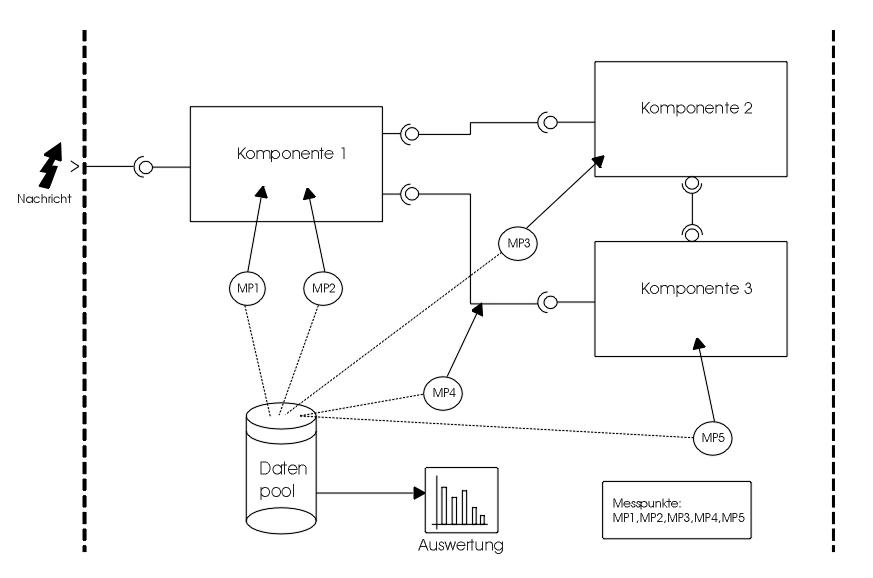
\includegraphics[width=13cm]{../res/simul.jpg}}
\caption{Schematische Darstellung der Simulation}
\label{pic:simul}
\end{center}
\end{figure}

\subsection{Ziele des Individuellen Projektes}
\label{sec:einleitung:ziele}
Ziel dieses Projektes ist die Erstellung einer Infrastruktur f�r die in Abschnitt \ref{sec:einleitung:motivation} erl�uterte Simulation in Form eines Frameworks. Bestandteil des Frameworks wird die Modellierung des Systems und der Komponenten, ein Modell zur Simulation von Anfragen an Dienste des Systems und die Auswertung der gesammelten Daten sein. Diese Bestandteile werden in einer Simulationsumgebung gekapselt.
\par
Bei der Entwicklung wird verst�rkt darauf geachtet, dass kleinere �nderungen und Erweiterungen des Frameworks nicht gro�e �nderungen der Implementierung zur Folge haben. So ist es beispielsweise w�nschenswert, dass einige sich von Modell zu Modell h�ufig �ndernde Bestandteile austauschen lassen, ohne eine Zeile Quellcode des Frameworks �ndern zu m�ssen. Weiterhin sollen Entwurfsentscheidungen, die die Umsetzung einer neuen Modellierung verhindern, �nderbar sein. Das bedeutet, dass die Bestandteile des Frameworks unabh�ngig voneinander austauschbar sein m�ssen.
\par
Das Projekt gliedert sich in die drei im Proposal \cite{lit:proposal} angegebenen Entwicklungsinkremente. Am Ende jedes Inkrementes wird ein der Entwicklungsstufe angepasster Prototyp entstehen, welcher das Framework in seinem aktuellen Stand benutzt.

\subsection{Aufbau dieser Ausarbeitung}
\label{sec:einleitung:aufbau}

Die Ausarbeitung gliedert sich in drei inhaltliche Teile, welche von dieser Einleitung und einem abschlie�enden Fazit eingeschlossen sind.
\par
Der erste Teil befasst sich mit der Kl�rung theoretischer Fragen in Bezug auf die Modellierung von Komponentenarchitekturen und der Simulation. Hierzu werden anf�nglich einige Grundlagen zur Modellierung von Komponenten erarbeitet, welche als Ziel das Modell der gesamten Komponentenarchitektur haben. Darauf aufbauend werden in diesem Modell potentielle Zeitverbraucher identifiziert. Der letzte Teil dieses Kapitels stellt das f�r das Framework entwickelte Simulationsmodell vor.
\par
Der zweite und gleichzeitig gr��te Teil dieser Ausarbeitung ist dem Entwurf des Frameworks gewidmet. Dieser beginnt mit dem Festlegen einiger allgemeiner Anforderungen an das Framework. Der zweite Teil dieses Kapitels erarbeitet eine sinnvolle Architektur des Frameworks. Das bedeutet, dass an dieser Stelle das Framework in seine groben Bestandteile gegliedert wird. Innerhalb dieser Teile werden dann unter Betrachtung von speziellen an den jeweiligen Teil gestellten Anforderungen einzelne Komponenten identifiziert. Der dritte Teil des Entwurfs bildet dann schlie�lich die Architektur mit ihren Komponenten auf Klassen und Pakete ab. Hier werden einige der Entwurfsentscheidungen zum besseren Verst�ndnis des Frameworks detailiert erkl�rt.
\par
Das dritte und abschlie�ende inhaltliche Kapitel der Ausarbeitung geht auf die Anwendung des Frameworks ein. Hierzu wird anhand eines Beispiels die Benutzung der Basisfunktionalit�t beschrieben. Weiterhin wird auf die Erweiterungsm�glichkeiten und deren Ansatzpunkte im Framework eingegangen. Um den Umfang der Funktionalit�t des Frameworks einsch�tzen zu k�nnen, wird dem Leser abschlie�end ein �berblick �ber die Grenzen des Frameworks vermittelt.
\newpage

\section{Modellbildung}
\label{sec:modell}
In diesem Kapitel wird auf die Entwicklung und Auswahl der im Framework verwendeten Modelle eingegangen. Hierzu geh�rt die Abbildung der Komponenten und der Architektur in ein Modell, die Identifizierung der Zeitverbraucher innerhalb der Architektur und die darauf aufbauende Modellierung der eigendlichen Simulation.

\subsection{Grundlagen zur Modellierung von Komponenten und Komponentenarchitekturen}
\label{sec:modell:grundlagen}
Da sich dieses Framework mit der Simulation von Modellen von Architekturen und Komponenten befassen soll, gilt es als erstes, geeignete Modelle f�r die Komponenten und die Architektur auszuw�hlen und diese ggf. f�r die Simulation anzupassen. Als Basis hierf�r wird auf ein Komponentenmodell zur�ckgegriffen, welches in \cite{lit:reussner01} vorgestellt wird. In diesem Modell repr�sentieren sich Komponenten durch eine Reihe angebotener Dienste. Diese Dienste werden nach au�en hin durch Schnittstellen (in \cite{lit:reussner01} als {\em Angebotssschnittstellen} bezeichnet) abgebildet. Die Dienste selber k�nnen andere m�glicherweise externe Dienste zu ihrer Ausf�hrung ben�tigen, welche ebenso durch Schnittstellen (in \cite{lit:reussner01} als {\em Bedarfsschnittstelle} bezeichnet) nach au�en abgebildet werden.

\subsubsection{Auswahl des Schnittstellenmodells}
\label{sec:modell:grundlagen:schnittstellen}
Das Modell sieht je nach Anfordung unterschiedliche Schnittstellenmodelle vor, welche hierarchisch angeordnet sind. Die aus \cite{lit:reussner01} entnommene Auflistung erl�utert diese kurz.
\begin{itemize}
\item \textbf{Signaturlisten} beschreiben die Signaturen von Diensten. Dazu geh�ren Name, Parameterzahl, Parametertypen und ggf. der R�ckgabetyp des Dienstes
\item \textbf{Protokolle} spezifizieren Reihenfolgen von Dienstaufrufen. Damit wird die Verf�gbarkeit von Diensten einer Komponente in Abh�ngigkeit ihres internen Zustands beschrieben sowie die Reihenfolgen, mit denen die Komponente externe Dienste aufrufen kann.

\item \textbf{Qualit�tsattribute und Nicht-funktionale Eigenschaften} betreffen Randbedingungen, die spezifizieren wie eine Komponente ihre Funktionalit�t erf�llt. Solche Randbedingungen betreffen beispielsweise Zuverl�ssigkeit, Effizienz bestimmter Dienste oder Robustheit.

\end{itemize}

Da im Framework die Komponenten nicht als Blackboxes simuliert werden sollen, ben�tigen die Schnittstellen selber keine Beschreibung der Nicht-funktionalen Eigenschaften der Komponente. Diese werden, wie in Abschnitt \ref{sec:modell:bestandteile} erl�utert, direkt im Modell der Dienste der Komponenten umgesetzt. Auf die Modellierung von Protokollen kann ebenfalls verzichtet werden, da die Simulation nicht dazu dient, Interoperabilit�t zu pr�fen. Es wird bereits davon ausgegangen, dass die Komponenten der zu simulierenden Architektur zusammenpassen. Somit gen�gt es, die unterste Ebene der Schnittstellenmodelle, die Signaturlisten, zu verwenden.


\subsubsection{Modellierung der Dienste}
\label{sec:modell:grundlagen:dienste}
Die Dienste einer Komponente werden in \cite{lit:reussner01} durch endliche Automaten (dort {\em Dienstbedarfautomaten} genannt) umgesetzt, wobei die Zust�nde einen Kontrollfluss unabh�ngig von anderen Diensten repr�sentieren und die Transitionen die Aufrufe anderer m�glicherweise externer Dienste darstellen. Ist ein Zustand als Endzustand definiert, so wird dies als Beendigung eines Dienstes (durch Erfolg oder Ausnahme) gewertet. Verlassen zwei Transitonen einen Zustand, so repr�sentiert dieses einen Zweig im Kontrollfluss, welcher in der Simulation durch an den Transitionen befindlichen Wahrscheinlichkeiten aufgel�st wird.
Bild \ref{pic:modell} zeigt einen Dienstbedarfsautomaten (f�r Dienst e0). Dieser k�nnte folgenden Quellcode einer Komponente modellieren.\\
\begin{code}
be\=gi\=n \=e0\=()\\
\>{\em interne Befehle}\\
\>if ({\em Bedingung})\\
\>\>e1();\\
\>\>{\em interne Befehle}\\
\>\>e2();\\
\>else \\
\>\>e3();\\
end e0

\end{code}

\subsubsection{Verbindungen zwischen Komponenten}
\label{sec:modell:grundlagen:verbindung}

Nachdem nun einzelne Komponenten modelliert werden k�nnen, m�ssen jetzt M�glichkeiten geschaffen werden, mehrere dieser Komponenten untereinander oder mit der Aussenwelt zu verbinden. Bei der Verbindung zweier Komponenten untereinander wird eine Bedarfsschnittstelle einer Komponente mit der Angebotsschnittstelle einer anderen verbunden. Bei der Verbindung zur Au�enwelt dagegen werden zwei Bedarfs- bzw. Angebotsschnittstellen miteinander verbunden. Die erste der beiden Verbindungen werden im Folgenden als ComponentMapping und die zweite als ComponentBinding bezeichnet. Abbildung \ref{pic:modell} stellt diesen Unterschied anschaulich dar.
\par
Da Schnittstellen unter Umst�nden mehrere Dienste kapseln, m�ssen innerhalb einer dieser Verbindungen Strukturen zur Verf�gung stehen, die jeden einzelnen Dienst verbinden. Diese Einzelverbindungen werden im Folgenden als Mapping bzw. Binding bezeichnet.

\begin{figure}[ht]
\begin{center}
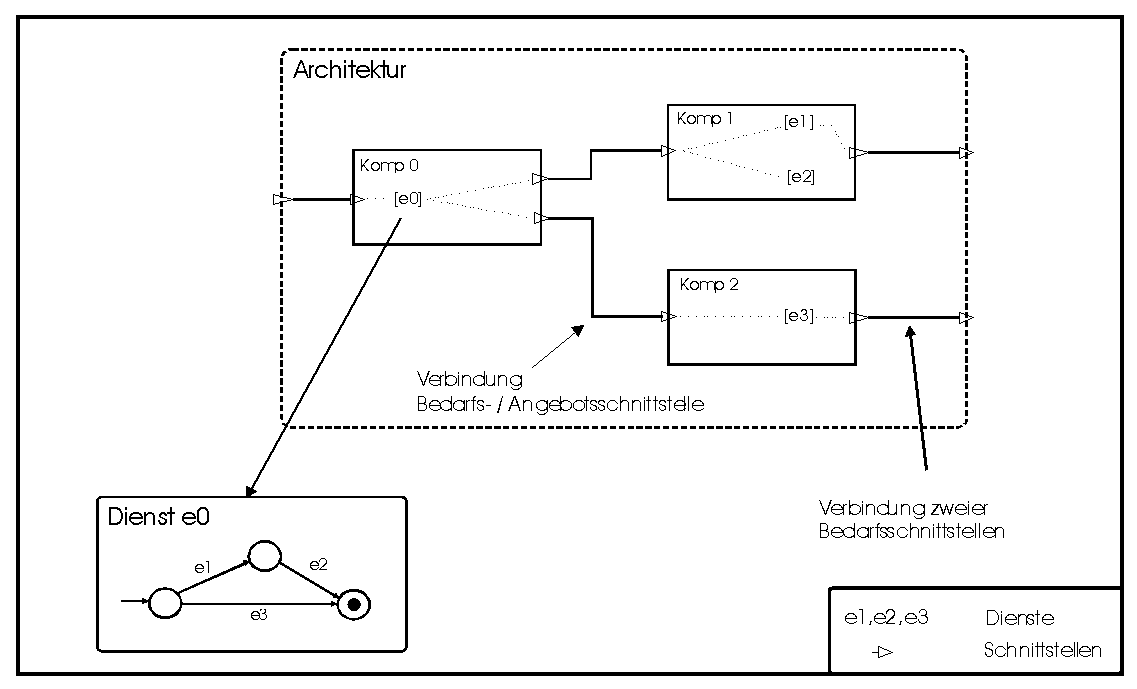
\includegraphics[width=13.5cm]{../res/modell.png}
\caption{Modell einer Komponentenarchitektur}
\label{pic:modell}
\end{center}
\end{figure}


\subsection{Identifizierung von zeitverbrauchenden Bestandteilen des Modells}
\label{sec:modell:bestandteile}
Nachdem im vorherigen Abschnitt die Modellierung einer Komponente beschrieben wurde, m�ssen nun innerhalb des Modells Zeitverbraucher identifiziert werden, welche der Simulation sp�ter als Datenbasis dienen werden. Hierzu hangeln wir uns im Modell durch den Kontrollfluss einer Anfrage.
\par
Dieser beginnt f�r gew�hnlich am Rand einer Architektur durch den Aufruf eines Dienstes, welcher �ber ein Binding innerhalb eines ComponentBinding in einer Komponente erreichbar ist. Ist diese �ber z.B. einen Softwarebus erreichbar, ergibt sich hier ein m�glichweise sogar dynamischer Zeitverbraucher. Es ist davon auszugehen, das alle Bindings innerhalb eines ComponentBinding die gleichen Laufzeiteigenschaften haben, da ein ComponentBinding ein Interface repr�sentiert und dieses f�r alle dort deklarierten Dienste den gleichen Weg nehmen wird. Somit gibt ein ComponentBinding eine dynamische Zeit vor, die alle enthaltenen Bindings benutzen k�nnen. Ebenso wie bei ComponentBindings verh�lt es sich bei der Verbindung zweier Komponenten, also bei ComponentMappings.
\par
Erreicht die Anfrage das Angebotsinterface, steht ihr als n�chstes der Weg zum Dienstbedarfsautomat bevor. Hierbei handelt es sich jedoch um einen Weg, welcher �blicherweise nur im Modell existiert. In der Realit�t ist ein Dienst f�r gew�hnlich eine Implementierung einer Methode eines Interface. Somit ist dieser Weg kein Zeitverbraucher. Soll trotzdem an dieser Stelle eine Zeitverz�gerung modelliert werden, so ist es prinzipiell m�glich, diese in den  Dienst einzurechnen.
\par
Dienste werden, wie in Abschnitt \ref{sec:modell:grundlagen:dienste} beschrieben, durch Dienstbedarfsautomaten also endliche Automaten modelliert, wobei Zust�nde interne Befehle und Transitionen externe Dienste repr�sentieren. Interne Befehle ben�tigen Rechenzeit, die sich auch wieder dynamisch �ndern kann, kommen also als dynamische Zeitverbraucher in Betracht. Externe Dienstaufrufe sind keine direkten Zeitverbaucher. Ihre Zeit berechnet sich aus dem Zeitverbauch des aufzurufenden Dienstes und dem Weg dahin.
\par
Nachdem nun alle Zeitverbraucher entlang dem Kontrollfluss einer Anfrage identifiziert wurden, besch�ftigt sich der n�chste Abschnitt mit dem Aufbau eines Simulationsmodells.

\subsection{Aufbau des Simulationsmodells}
\label{sec:modell:simulation}

Beim Entwurf des Simulationsmodell geht es darum, an die Architektur gestellte Anfragen und deren Wechselwirkungen innerhalb der Architektur m�glichst realit�tsnah zu simulieren. Es kommen grunds�tzlich zwei M�glichkeiten in Frage, die im n�chsten Abschnitt kurz diskutiert werden.

\subsubsection{Reelle Threads vs. simulierte Threads}
\label{sec:modell:simulation:reellvssim}

Bei der Simulation mit reellen Threads wird f�r jede Anfrage an das System ein reelles Thread erzeugt. Wie in der Realit�t auch, werden diese an bestimmten Stellen in der Architektur Zeit verbrauchen. Dies l��t sich erreichen, indem die Threads an diesen Stellen f�r eine bestimmte Zeit blockiert werden. Diese Zeit kann im einfachsten Fall der Realit�t entsprechen, was dazu f�hrt, dass das Modell in Echtzeit arbeitet. Nachteile bei dieser Methode ergeben sich, wenn sowohl kurze als auch lange Verz�gerungszeiten in der Architektur auftreten, da sich dann m�glicherweise eine unn�tige Wartezeit ergibt. Diese k�nnte man �berbr�cken, indem die Simulationszeit gezielt  vorgestellt wird. Als erheblicher Nachteil bei diesem Prinzip erweist sich jedoch die Sychronisation der einzelnen Threads insbesondere wenn sie gleichzeitig an der selben Stelle auftreten. Experimentelle Versuche erwiesen hier aufgrund eben genannter Problematik komplizierte schlecht erweiterbare Konstrukte. Aufgrund dieser Nachteile, insbesondere der Synchronisationsproblematik, wird von der Verwendung dieses Ansatzes abgesehen. 
\par
Der zweite Ansatz simuliert Threads. Hierzu werden Stellen innerhalb der Architektur mit einer Zeit markiert. Die simulierten Threads starten an einer dieser Stellen und addieren dann die Zeiten entlang ihres Kontrollflusses auf. Somit wird die Zeit der Simulation unabh�ngig von der Architektur, da die zu verbrauchende Zeit nicht verstreichen muss. Dieser Ansatz gestattet problemlos die Verarbeitung mehrer Anfragen, solange der Durchlauf einer Anfrage keinerlei Einfluss auf den  Kontrollfluss oder die zeitverbrauchenden Bestandteile der Architektur mit sich bringt. Ein solches Modell spiegelt jedoch die Realit�t nicht gut wieder. Es ist beispielsweise w�nschenswert, bei der Modulation einer Single-Thread-Komponente die Wartezeit einer Anfrage zu erh�hen, wenn gerade eine andere Anfrage verarbeitet wird. Auf diese Art lassen sich ebenfalls Auslastungen des Prozessors, auf dem die Komponente l�uft, modellieren. Weiterhin sinnvoll erscheint die dynamische �nderung des Kontrollflusses. Folgendes Beispiel erl�utert den Sinn dieser Modellierung.
\par
Soll das Modell eine Schleife im Kontrollfluss modellieren, so benutzt man folgenden Ansatz. Man modelliert wie in Bild \ref{pic:rekurs} dargestellt eine Endlosschleife, wobei 1.0 und 0.0 die, wie in Kapitel  \ref{sec:modell:grundlagen:dienste} beschrieben, Wahrscheinlichkeiten zur Aufl�sung des Zweiges darstellen. Soll die Schleife nach einigen Durchl�ufen abgebrochen werden, so m�ssen diese Wahrscheinlichkeiten in Abh�ngigkeit der Anzahl der Durchl�ufe ver�ndert werden, damit die Schleife verlassen wird.

\begin{figure}[ht]
\begin{center}
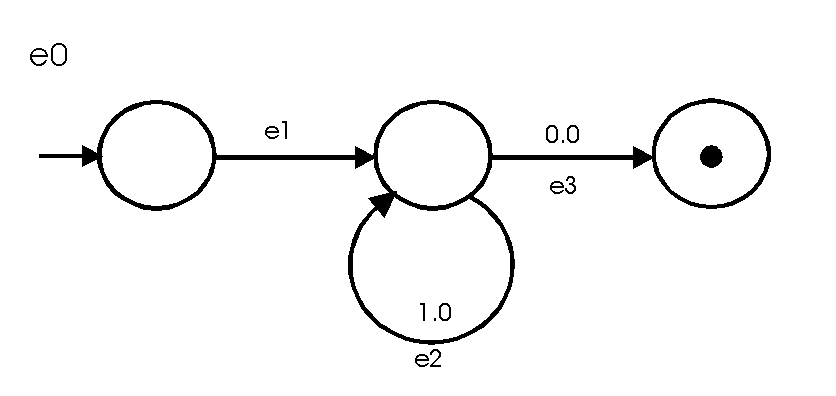
\includegraphics[width=7cm]{../res/rekurs.png}
\caption{Dienstbedarfsautomat moduliert eine Endlosschleife}
\label{pic:rekurs}
\end{center}
\end{figure}

Um diese beiden Anforderungen im Simualtionsmodell unterzubringen, ist auch in diesem Fall die Synchronisation der Anfragen untereinander notwendig, damit diese ihren gleichzeitigen Aufenthalt an ein und der selben Stelle in der Architektur �berhaupt wahrnehmen k�nnen. Hierbei kommt man schnell zu der Erkenntnis, dass das einfache aufaddieren der Zeiten hier nicht mehr gen�gt, da das Einrechnen der Wechselwirkungen durch andere Threads unm�glich ist. Eine kleine Modifikation des Ansatzes l�st dieses Problem. Die Simulation wird pro Anfrage nicht mehr am St�ck durchgef�hrt, sondern Schrittweise. Dies bedeutet, dass alle zur Zeit vorhandenen Anfragen um die gleiche Schrittweite vorgestellt werden. Nun ist die dynamische Anpassung der Wartezeiten problemlos m�glich, da alle Anfrage quasi gleichzeitig simuliert werden. Die maximale Schrittweite eines Schrittes ist hierbei begrenzt durch die Zeit, in der keines der Threads eine Zustands�nderung erf�hrt. Mit Zustands�nderung sei hier der Wechsel eines Threads zum n�chsten zeitverbrauchenden Bestandteil der Architektur im Kontrollfluss gemeint. Der folgende Abschnitt verdeutlicht die Umsetzung dieses Ansatzes anhand eines Beispiels.

\subsubsection{Ablauf einer Simulation}
\label{sec:modell:simulation:sync}

In Bild \ref{pic:ablauf} ist eine m�gliche Startkonfiguration einer Simulation dargestellt. Es befinden sich zum Zeitpunkt 0 drei Anfragen an bestimmten Punkten des Systems. Entlang der Zeitachse t sind f�r jedes Thread die Wartezeiten eingetragen, welche hier der Einfachheit halber statisch gew�hlt sind. 

\begin{figure}[ht]
\begin{center}
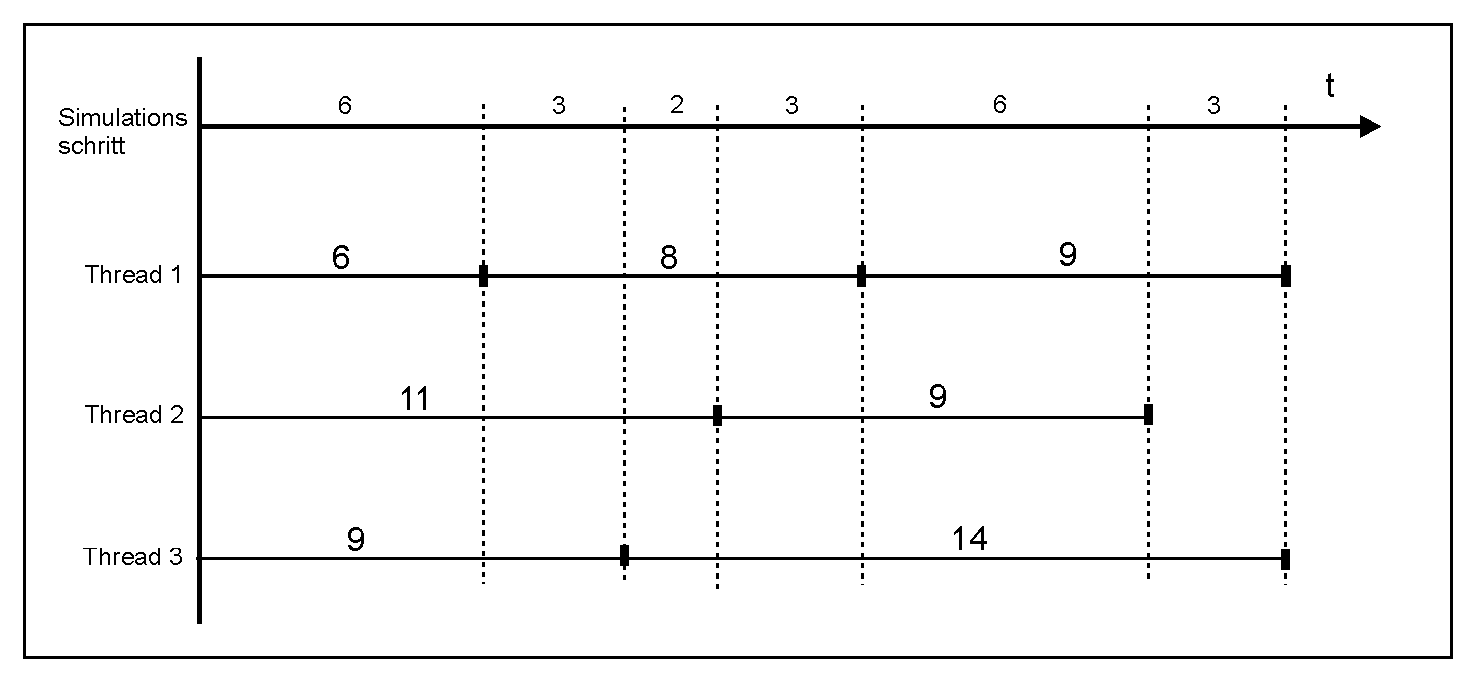
\includegraphics[width=13cm]{../res/simmodell.png}
\caption{Simulation von Anfragen}
\label{pic:ablauf}
\end{center}
\end{figure}

Der n�chste Zeitschritt berechnet sich aus der k�rzesten noch verbleibenden Wartezeit aller Threads, im Beispiel also 6, da nach Ablauf dieser Zeit Thread 1 seinen Zustand �ndert. Wird der Zeitschritt ausgef�hrt, so verringert sich bei allen Threads die verbleibende Zeit um diesen Schritt. Erreicht ein Thread eine verbleibende Zeit von 0, so wechselt dieses zu seinem n�chsten Zeitverbraucher im Kontrollfluss. Existiert dieser nicht, so hat das Thread die Abarbeitung der Anfrage beendet. In Bild \ref{pic:ablauf} erreicht beispielsweise Thread 2 diesen Zustand nach 20 Zeiteinheiten. Nachdem alle Threads diesen Zustand erreicht haben, im Beispiel nach 23 Zeiteinheiten, endet die Simulation.\\

\par
Nachdem in diesem Kapitel die theoretischen Hintergr�nde f�r die Simulation von Komponentarchitekturen ausgibig diskutiert wurden, befasst sich das n�chste Kapitel mit der praktischen Umsetzung dieser Modelle.
\newpage


\end{document}